\documentclass{article}

\usepackage{amsmath,amsfonts,amssymb,mathtools} % formatting math
\usepackage{amsthm} % for proofs
\usepackage{verbatim} % for block comments
\usepackage{hyperref} % for links

\hypersetup{
    colorlinks=true,
    linkcolor=blue,
    filecolor=magenta,      
    urlcolor=blue,
}

%+++++++++++++++++++++++++++++++

% FANCY LETTERS
\newcommand{\R}{\mathbb{R}} % the real number R
\newcommand{\E}{\mathbb{E}} % expectation symbol E

% BRACKETS, PARENTHESIS, AND CURLY BRACKETS
\newcommand{\lb}{\left[} % left bracket
\newcommand{\rb}{\right]} % right bracket
\newcommand{\lp}{\left(} % left parenthesis
\newcommand{\rp}{\right)} % right parenthesis
\newcommand{\lc}{\left\{} % left curly bracket
\newcommand{\rc}{\right\}} % right curly bracket

\title{Geometric Data Analysis HW 1}
\author{Gilad Turok, gt2453 \\ \href{mailto:gt2453@columbia.edu}{gt2453@columbia.edu}}
\date{\today}

\begin{document}
\maketitle

\section[]{$k$-means vs Single-Linkage Clustering}

    I generated data with three $2$-dimensional Gaussians with identity convariance matricies. I cluster this data with $k$-means and single-linkage clustering with means that vary. I use $4$ different sets of means, beginning from very close to each other to further and further apart:

    \begin{align*}
        \mu_1 = \begin{bmatrix} 0 \\ 0 \end{bmatrix}, \quad \mu_2 = \begin{bmatrix} 0 \\ 0 \\ \end{bmatrix}, \quad \mu_3 = \begin{bmatrix} 0 \\ 0 \end{bmatrix} \\
        \mu_1 = \begin{bmatrix} -2 \\ 2 \end{bmatrix}, \quad \mu_2 = \begin{bmatrix} 0 \\ -2 \end{bmatrix}, \quad \mu_3 = \begin{bmatrix} 2 \\ 2 \end{bmatrix} \\
        \mu_1 = \begin{bmatrix} -5 \\ 5 \end{bmatrix}, \quad \mu_2 = \begin{bmatrix} 0 \\ -5 \end{bmatrix}, \quad \mu_3 = \begin{bmatrix} 5 \\ 5 \end{bmatrix} \\
        \mu_1 = \begin{bmatrix} -10 \\ 10 \end{bmatrix}, \quad \mu_2 = \begin{bmatrix} 10 \\ -10 \end{bmatrix}, \quad \mu_3 = \begin{bmatrix} 10 \\ 10 \end{bmatrix} \\
    \end{align*}

    The $k$-means algorithm is very sensitive to initialization of cluster centers while single-linkage clustering is not -- it converges to the same result. When the means are all the same, i.e. $\mu_1 = \mu_2 = \mu_3 = 0$, the true clusters are all on top of each other, as shown in the top left plot. $k$-means clusters this into $3$ clusters while single-linkage clustering places nearly all data points in one cluster. In general, when the means are close together, single-linkage clustering often collapses into one entire cluster while $k$-means does not.

    \begin{figure}[ht]
        \label{fig:kmeans_singlelinkage}
        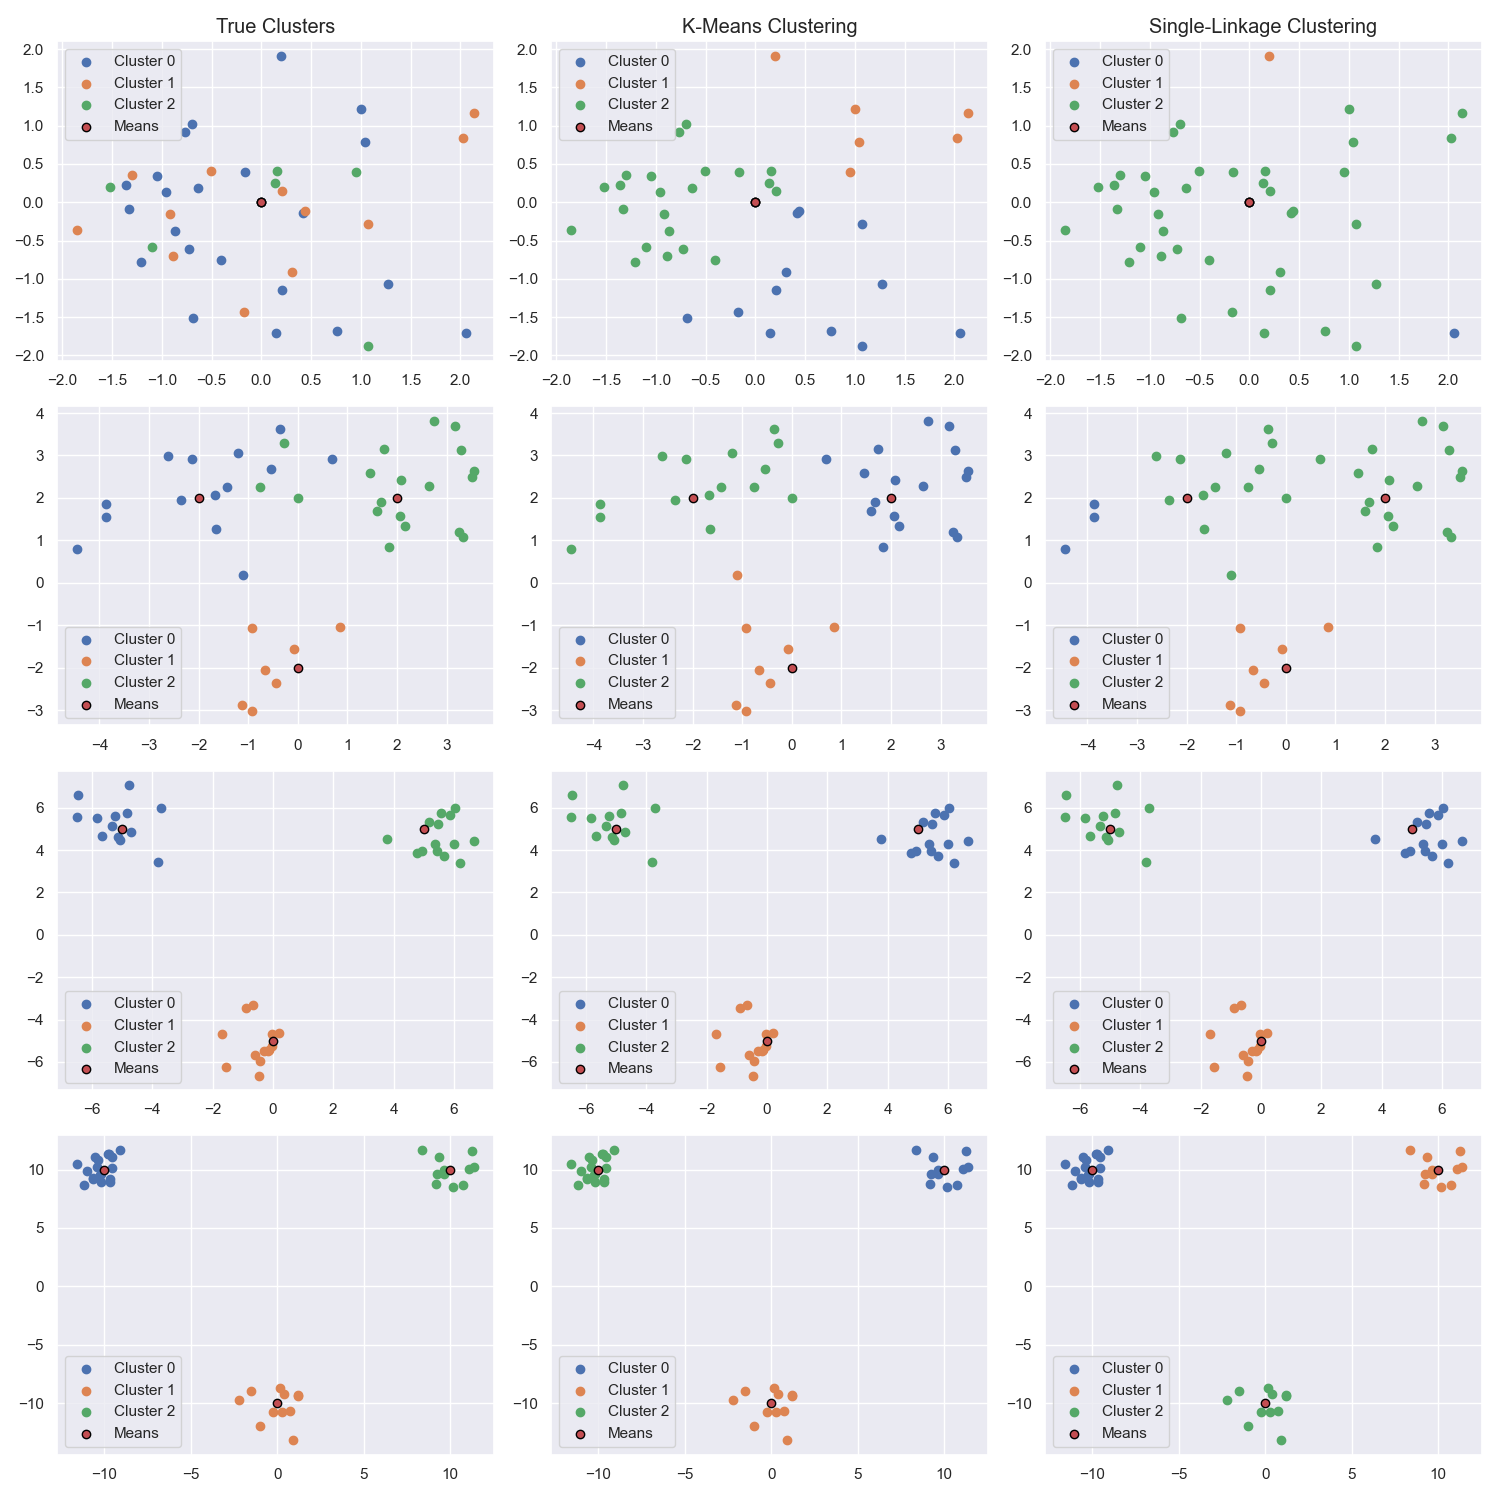
\includegraphics[width=0.99\linewidth]{images/q1/kmeans_singlelinkage.png}
        \caption{$k$-means vs single-linkage clustering on $3$ Gaussians with means at different distances}
    \end{figure}
    \pagebreak

\section[short]{$k$-means Clustering With Noise}

    \subsection[short]{Gaussian Noise}

        I added Gaussian noise $\mathcal{N}(0, \sigma^2)$ to my data $\mathbf{X}$. I plot the true clusters and set $\sigma^2$ to the following values: $0, 0.5, 1, 2, 5$. When $\sigma^2=0$, $k$-means performs well, correctly clustering nearly all the data points. However, as the noise increases, $k$-means becomes less and less accurate. Due to the random intialization of the means, $k$-means is very sensitive to noise -- this is why multiple runs of $k$-means is often recomemended.
        
        \begin{figure}[ht]
            \label{fig:kmeans_gaussian_noise}
                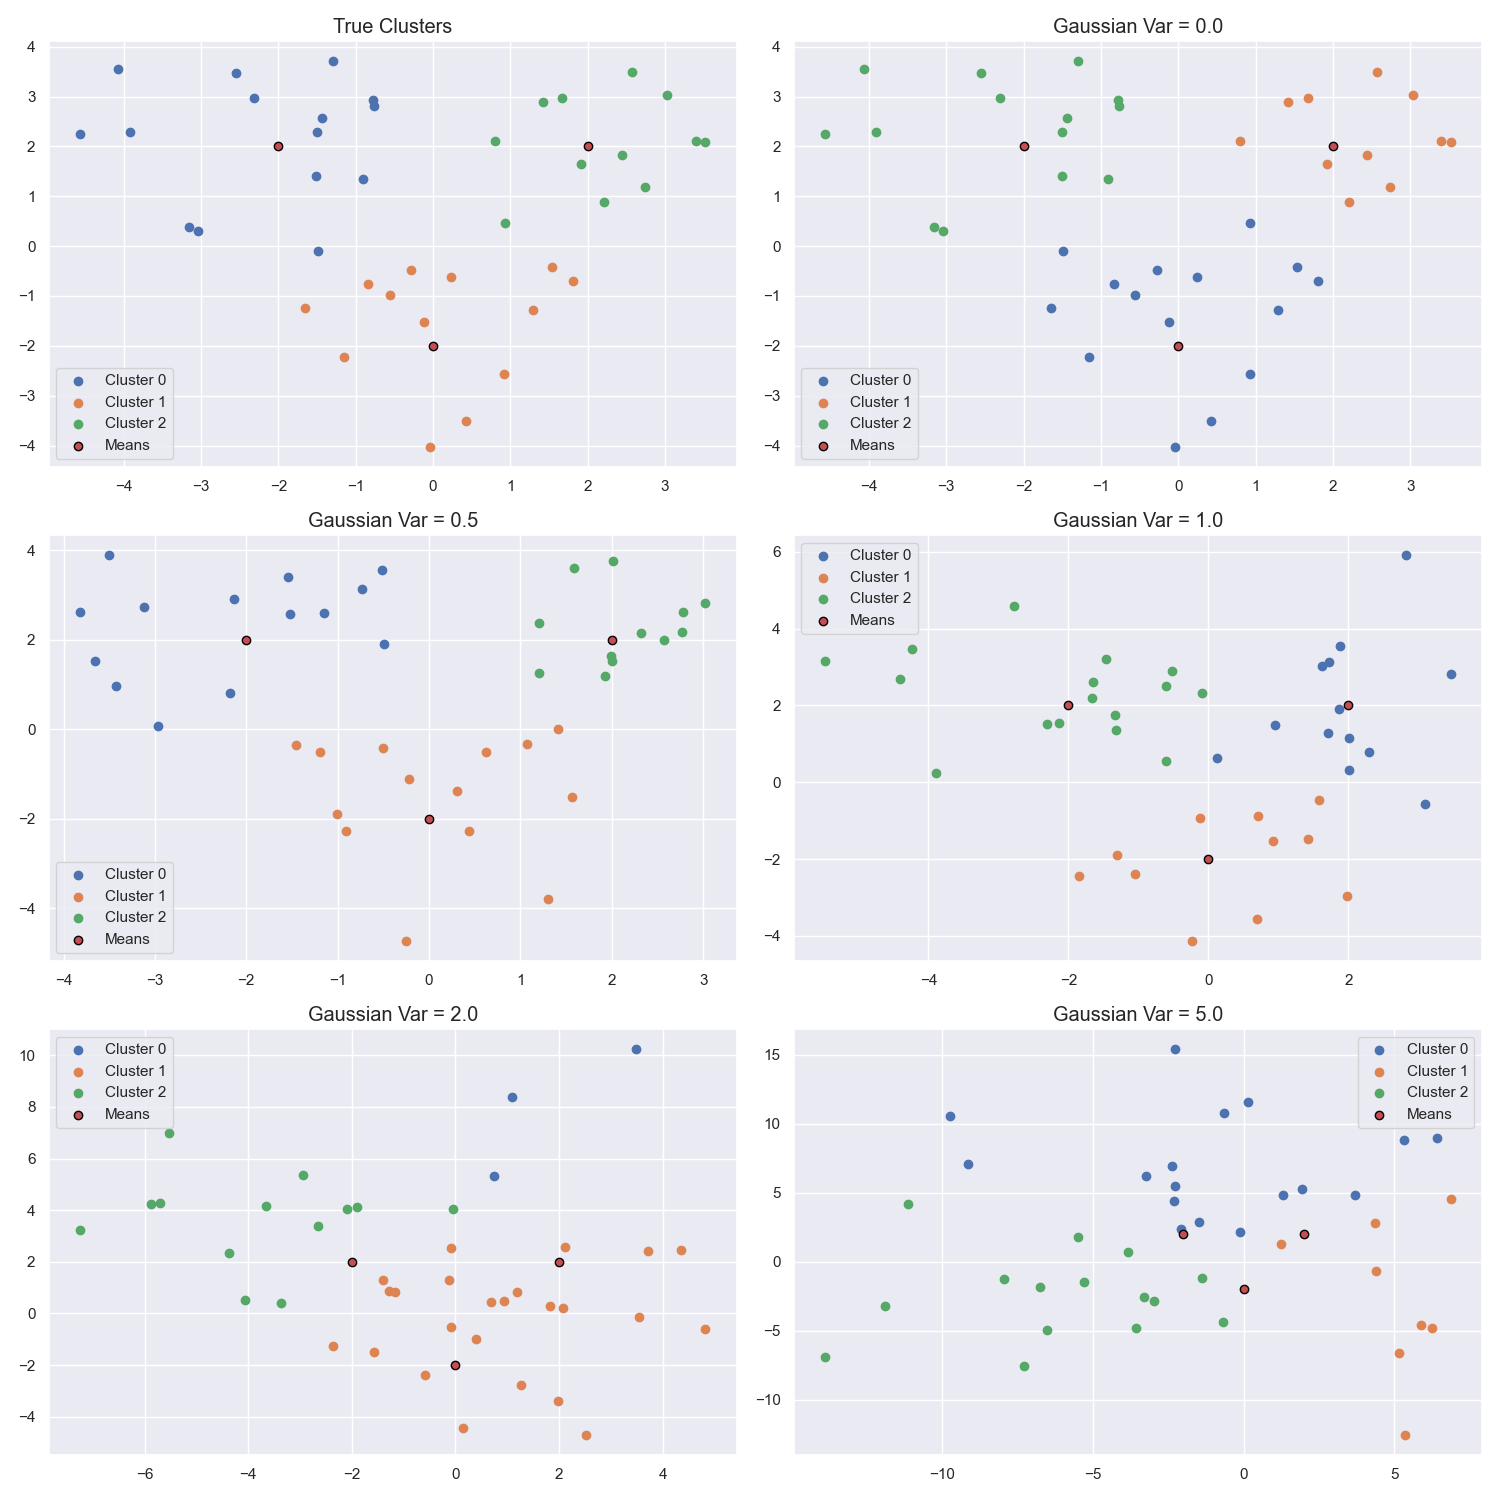
\includegraphics[width=0.99\linewidth]{images/q2/gaussian_noise.png}
                \caption{$k$-means with increasing amounts of Gaussian noise}
            \end{figure}
            \pagebreak

    \subsection[short]{Adversarial Noise}

        Adversial noise in single-linkage clustering can be used to create a "bridge" between two clusters that are otherwise far apart. In $k$-means clustering, for a given cluster-center initialization, adversarial points may also sometimes create a "bridge" that slowly shifts the cluster center towards the adversarial point as the algorithm converges. However, this problem is much severe than in the case of single-linkage clustering. Furthermore, adversarial noise can be used to place all $L$ data points into their own cluster which $k$-means would miss.

\section[short]{Hierarchial $k$-Means and $k$-Medians}

        One can make a hierarchial version of $k$-means or $k$-medians as $k$ varies. There are multiple ways to do so, but I will elaborate upon one such way. Let there be $k$ desired clusters and $n$ data points $x_1 \ldots x_n$.

        Hierarchial clustering e.g. single-linkage clustering suffers from expenstive computational overhead. If one knows the general range of desired clusters, i.e. $k=[4,10]$, hierarchial clustering begins from $k=n$, where $n$ can be tens or hundreds of thousands of data points. Instead, one can run $k$-means or $k$-medians with $k=10$ and merge the nearest clusters as per single-linkage clustering. This would allow one to more efficeintly create a dendrogram with only $k=[4,10]$, for example. However, to ensure robustness, one would want to initialize $k$-means and $k$-medians multiple times and compare the results.

\section[short]{Clustering Data With $k$-means and \\ Single-Linkage Clustering}
             

\end{document}